\documentclass{article}
\usepackage{array, booktabs, graphicx, apacite, setspace}
\usepackage[titletoc,toc,title]{appendix}
\usepackage[toc,section=section]{glossaries}
\usepackage{tocloft}
\usepackage{titlesec}


% set section indentation
\setcounter{secnumdepth}{4}


% add space between paragraphs
\setlength{\parskip}{\baselineskip}


% format \paragraph{example} as a subsubsubsection
\titleformat{\paragraph}
{\normalfont\normalsize\bfseries}{\theparagraph}{1em}{}
\titlespacing*{\paragraph}
{0pt}{3.25ex plus 1ex minus .2ex}{1.5ex plus .2ex}


% automatically convert "" to ``''
\usepackage [autostyle, english = american]{csquotes}
\MakeOuterQuote{"}


% define list of equations
\newcommand{\listequationsname}{\Large{List of Equations}}
\newlistof{myequations}{equ}{\listequationsname}
\newcommand{\myequations}[1]{
   \addcontentsline{equ}{myequations}{\protect\numberline{\theequation}#1}
}
\setlength{\cftmyequationsnumwidth}{2.3em}
\setlength{\cftmyequationsindent}{1.5em}


% format appendix numbering
\renewcommand\appendix{\par
  \setcounter{section}{0}
  \setcounter{subsection}{0}
  \setcounter{figure}{0}
  \setcounter{table}{0}
  \renewcommand\thesection{Appendix \Alph{section}}
  \renewcommand\thefigure{\Alph{section}\arabic{figure}}
  \renewcommand\thetable{\Alph{section}\arabic{table}}
}


% -------- GLOSSARY ENTRIES -------- %
\makenoidxglossaries

\newglossaryentry{word}{
	name={Word},
	description={Definition of the word}
}


% renames "Contents" to "Table of Contents"
\renewcommand\contentsname{Table of Contents}

\begin{document}

% -------------------------------------- %
% ------------ FRONT MATTER ------------ %
% -------------------------------------- %

% -------- TITLE PAGE -------- %

\title{\huge Report Title \\ \Large \medskip Subtitle}
\author{Charles Clayton}
\date{\today}
\maketitle
`
\thispagestyle{empty}

\pagenumbering{roman}
\setcounter{page}{0}


% -------- TABLE OF CONTENTS/LISTS -------- %

\singlespacing			\pagebreak
\tableofcontents		\pagebreak

\listoffigures		
\listoftables
\listofmyequations
\pagebreak


% -------- GLOSSARY -------- %

\printnoidxglossaries	\pagebreak


% ----------------------------- %
% -------- MAIN MATTER -------- %
% ----------------------------- %

\pagenumbering{arabic}
\onehalfspacing

\section{Introduction}

Lorem ipsum dolor sit amet, consectetur adipiscing elit, sed do eiusmod tempor incididunt ut labore et dolore magna aliqua. Ut enim ad minim veniam, quis nostrud exercitation ullamco laboris nisi ut aliquip ex ea commodo consequat. 

Duis aute irure dolor in \gls{word} reprehenderit in voluptate velit esse cillum dolore eu fugiat nulla pariatur \cite{einstein}.


\subsection{Background}

Ut enim ad minim veniam, quis nostrud exercitation ullamco laboris nisi ut aliquip ex ea commodo consequat. Duis aute irure dolor in reprehenderit in voluptate velit esse cillum dolore eu fugiat nulla pariatur. 

\begin{table}[ht]
  \centering
  \caption{Table without vertical lines}
  \begin{tabular}{
  		>{\centering\bfseries}m{0.5in} 
  		>{\centering}m{1in} 
  		>{\centering}m{0.5in} 
  		>{\centering\arraybackslash}m{0.5in}
  		}
    \toprule
    Letter & \textbf{Date} & \textbf{Number} & \textbf{Note} \\ 
    \midrule
	$x$ & 5-Mar-2016 & 1 & do \\
	$y$ & 6-Feb-2016 & 2 & re \\
	$z$ & 7-Jun-2016 & 3 & mi \\
	\bottomrule
  \end{tabular}
\end{table}

Excepteur sint occaecat cupidatat non proident, sunt in culpa qui officia deserunt mollit anim id est laborum.

\section{Discussion} 

Duis aute irure dolor in reprehenderit in voluptate velit esse cillum dolore eu fugiat nulla pariatur. Excepteur sint occaecat cupidatat non proident, sunt in culpa qui officia deserunt mollit anim id est laborum.


\begin{equation}
\int_{0}^{2\pi} \rho^2 d\rho
\end{equation}
\myequations{Example equation}

\subsection{Design} 
Duis aute irure dolor in reprehenderit in voluptate velit esse cillum dolore eu fugiat nulla pariatur. Excepteur sint occaecat cupidatat non proident, sunt in culpa qui officia deserunt mollit anim id est laborum.


\subsubsection{Details}
Excepteur sint occaecat cupidatat non proident, sunt in culpa qui officia deserunt mollit anim id est laborum \cite{knuth-fa}.

\subsubsection{Schematic}

Duis aute irure dolor in reprehenderit in voluptate velit esse cillum dolore eu fugiat nulla pariatur. 

\begin{figure}[ht!]
\centering
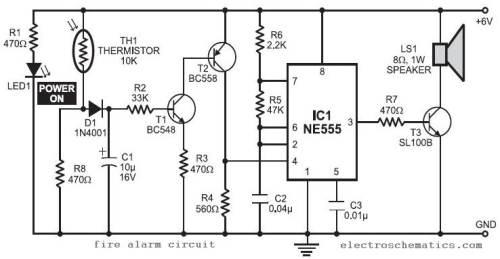
\includegraphics[width=80mm]{Images/schematic.png}
\caption{Schematic image}
\end{figure}

\section{Conclusion}

Lorem ipsum dolor sit amet, consectetur adipiscing elit, sed do eiusmod tempor incididunt ut labore et dolore magna aliqua. Ut enim ad minim veniam, quis nostrud exercitation ullamco laboris nisi ut aliquip ex ea commodo consequat.

% ----------------------------- %
% -------- BACK MATTER -------- %
% ----------------------------- %

% -------- BIBLIOGRAPHY -------- %
\clearpage
\doublespacing
\bibliography{references}
\bibliographystyle{apacite} 
\pagebreak

% -------- APPENDIX -------- %
\appendix
\onehalfspacing
\section*{Appendix}
\addcontentsline{toc}{section}{Appendix}
\renewcommand{\thesubsection}{\Alph{subsection}}

\subsection{Calculations}
Lorem ipsum dolor sit amet, consectetur adipiscing elit, sed do eiusmod tempor incididunt ut labore et dolore magna aliqua. Ut enim ad minim veniam, quis nostrud exercitation ullamco laboris nisi ut aliquip ex ea commodo consequat.


\end{document}